\documentclass[../main.tex]{subfiles}
% !TEX root= ../main.tex

\begin{document}

\begin{itemize}
	\item A sorting network is either the identity network or a sorting network, S composes with a \textbf{compare-and-swap module} such that two output of S are the inputs to the compare-and-swap, and the output of the compare-and-swap are output of the new sorting network.
\end{itemize}

\begin{center}
	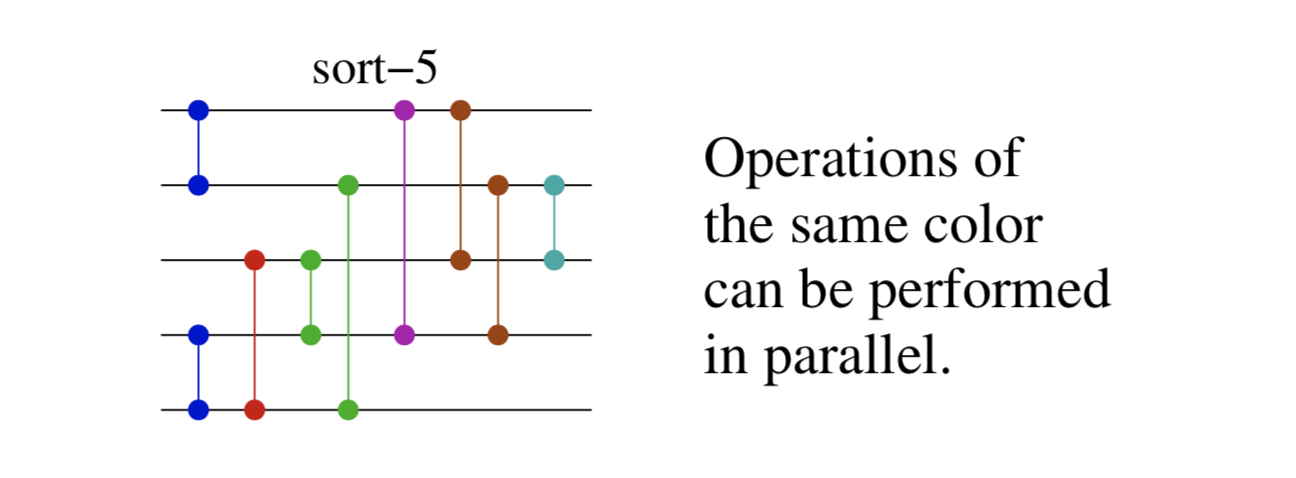
\includegraphics[scale=0.4]{work-flow-graph.png}
\end{center}

\begin{itemize}
	\item Each \textit{compare-and-swap} is a vertex of the work-flow graph.Z
	\item Connection between compare-and-swaps are edges in the work-flow graph.
	\item \textbf{Work:} number of compare-and-swap elements.
	\item \textbf{Span:} number of "levels" in the "most-compact" drawing of the network.
\end{itemize}

\subsection{The 0-1 Principle}

\begin{itemize}
	\item If a sorting network correctly sorts all inputs consisting only of 0s and 1s, then it correctly sorts inputs consisting of arbitrary values.
	\item \textbf{Monotonicity Lemma:}
	      \begin{itemize}
		      \item Let \(S\) be a sorting network with \(n\) inputs an \(N\) outputs.
		      \item Let \(f\) be any monotonic function, if \(x \leq y\), then \(f(x) \leq f(y)\).
		      \item \(S \circ f \equiv f \circ S\)
	      \end{itemize}
\end{itemize}

\subsubsection{Bitonic Merge}

\begin{itemize}
	\item Recursion assumption: input is two, \textbf{sorted} vectors of equal length.
	\item \textbf{Monotonic sequences:}
	      \begin{itemize}
		      \item A sequence is \textbf{monotonically increasing} if \(X_0 \leq X_1 \leq \cdots \leq X_{N-1}\).
		      \item A sequence is \textbf{monotonically decreasing} if \(X_0 \geq X_1 \geq \cdots \geq X_{N-1}\).
	      \end{itemize}
	\item \textbf{Bitonic Sequences:} A sequence is bitonic if it consists of a monotonically increasing followed by a monotonically decreasing sequence.
	      \begin{itemize}
		      \item Either of those sub-sequences can be empty.
		      \item Any subsequence of a bitonic sequence is bitonic.
	      \end{itemize}
	\item Let X be a monotonically increasing of 0s and 1s of length N.
	      \begin{align*}
		      Z_i & = \min(X_i, X_{i+\frac{N}{x}}) & 0           & \leq i < \frac{N}{2} \\
		      Z_i & = \max(X_{i-\frac{N}{2}}, X_i) & \frac{N}{2} & \leq i < N
	      \end{align*}
\end{itemize}

\subsection{Bitonic Sort}

\begin{itemize}
	\item Divide into two halves of size \(\frac{N}{2}\), \textbf{Parallel:} sort each half.
	\item Combine the two, sorted halves into one bitonic sequence of length \(N\).
	\item Create a clean (a sequence is all 0s or all 1s) half of length \(\frac{N}{2}\) and a bitonic half of length \(\frac{N}{2}\).
	      \begin{center}
		      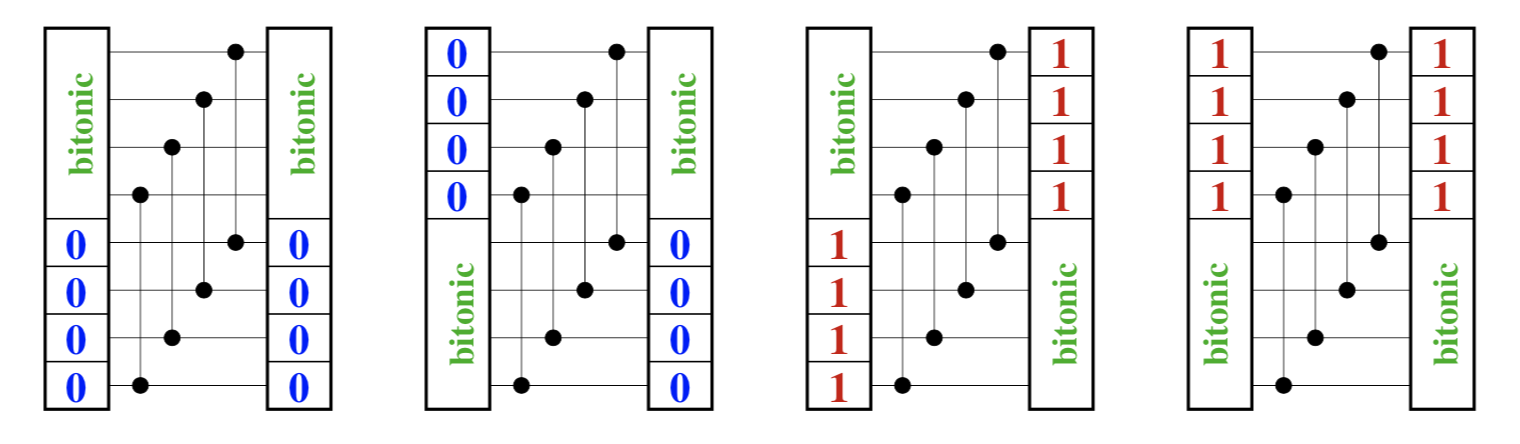
\includegraphics[scale=0.6]{bitonic-merge.png}
	      \end{center}
	\item Recursively merge the two halves, \textbf{Parallel:} marge each half.
	      \begin{itemize}
		      \item Total parallel time/\textbf{Span}: \(\log_2{N}\)
		      \item Total number of compare-and-swaps/\textbf{Work} \(\frac{N}{2}\log_2{N}\)
	      \end{itemize}
	\item \textbf{Complexity:}
	      \begin{itemize}
		      \item Total Parallel Time/\textbf{Span}: \(\sum_{k=1}\log_2{Nk} = O(\log^2{N})\)
		      \item Total Number of Compare-and-Swaps/\textbf{Work}: \(\sum_{k=1}\frac{N}{2}\log_2{N} = O(N\log^2{N})\)
	      \end{itemize}
\end{itemize}

\end{document}


